%%%%%%%%%%%%%%%%%%%%%%%%%%%%%%%%%%%%%%%%%
% Simple Sectioned Essay Template
% LaTeX Template
%
% This template has been downloaded from:
% http://www.latextemplates.com
%
% Note:
% The \lipsum[#] commands throughout this template generate dummy text
% to fill the template out. These commands should all be removed when 
% writing essay content.
%
%%%%%%%%%%%%%%%%%%%%%%%%%%%%%%%%%%%%%%%%%

%----------------------------------------------------------------------------------------
%	PACKAGES AND OTHER DOCUMENT CONFIGURATIONS
%----------------------------------------------------------------------------------------

\documentclass[12pt]{article} % Default font size is 12pt, it can be changed here

\usepackage{geometry} % Required to change the page size to A4
\geometry{a4paper} % Set the page size to be A4 as opposed to the default US Letter

\usepackage{graphicx} % Required for including pictures

\usepackage{float} % Allows putting an [H] in \begin{figure} to specify the exact location of the figure
\usepackage{listings}

\linespread{1.2} % Line spacing

%\setlength\parindent{0pt} % Uncomment to remove all indentation from paragraphs

\graphicspath{{.}} % Specifies the directory where pictures are stored
\newcommand{\tab}{\hspace*{2em}}

\begin{document}

%----------------------------------------------------------------------------------------
%	TITLE PAGE
%----------------------------------------------------------------------------------------

\begin{titlepage}

\newcommand{\HRule}{\rule{\linewidth}{0.5mm}} % Defines a new command for the horizontal lines, change thickness here

\center % Center everything on the page

\textsc{\LARGE Serpent Cipher}\\[1.5cm] % Name of your university/college
\textsc{\Large Final Report}\\[0.5cm] % Major heading such as course name
\textsc{\large Cryptography}\\[0.5cm] % Minor heading such as course title

\HRule \\[0.4cm]
{ \huge \bfseries Team Rikki-Tikki-Tavi}\\[0.4cm] % Title of your document
\HRule \\[1.5cm]

\begin{minipage}{0.4\textwidth}
\begin{flushleft} \large
\emph{Authors:}\\
Nicholas \textsc{Sereni} % Your name
\newline
Dan \textsc{Grau}
\newline
Karl \textsc{Berger}
\end{flushleft}
\end{minipage}
~
\begin{minipage}{0.4\textwidth}
\begin{flushright} \large
\emph{Prof.:} \\
Alan \textsc{Kaminsky} % Supervisor's Name
\end{flushright}
\end{minipage}\\[4cm]

{\large \today}\\[3cm] % Date, change the \today to a set date if you want to be precise

%\includegraphics{Logo}\\[1cm] % Include a department/university logo - this will require the graphicx package

\vfill % Fill the rest of the page with whitespace

\end{titlepage}

%----------------------------------------------------------------------------------------
%	TABLE OF CONTENTS
%----------------------------------------------------------------------------------------

\tableofcontents % Include a table of contents

\newpage % Begins the essay on a new page instead of on the same page as the table of contents 

%----------------------------------------------------------------------------------------
%	INTRODUCTION
%----------------------------------------------------------------------------------------

\section{Serpent Cipher} % Major section

%------------------------------------------------

\subsection{Background} % Sub-section
The Serpent cipher was designed by Ross Angerson, Eli Biham, and Lars Knudsen. It was created as candidate for the Advanced Encryption Standard. Based on AES requirements, it has a 128 bit block length and a 256 bit key length. It also supports keys sizes of 128 and 192 bits. 

%------------------------------------------------

\subsection{The Algorithm} % Sub-section
Serpent splits the 128 bit block into four 32-bit words. There are 32 rounds. Each round uses a subkey generated from the user key. The user key does not have a size requirement, but it becomes fixed at 128, 192, or 256 bits. Padding is achieved by appending a ``1" followed by ``0" bits. The algorithm can be summarized as:

\begin{itemize}
\item An initial permutation
\item 32 rounds consisting of:
\begin{itemize}
\item key mixing operation
\item S-boxes
\item linear transformation (replaced by a a key mixing operation in the final round)
\end{itemize}
\item A final permutation

This process is explained visually in Figure~\ref{fig:Block Diagram of Encryption}.


\end{itemize}
\begin{figure}[H]
\centering
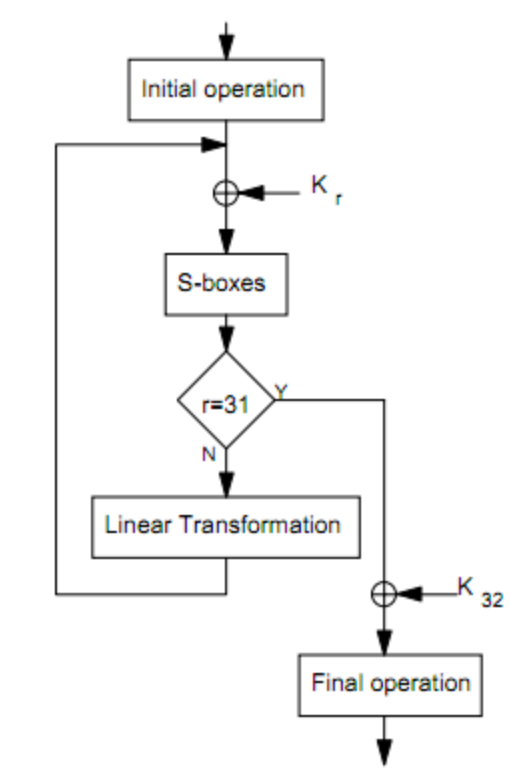
\includegraphics[width=5cm,height=7cm]{encryption}
\caption{Block Diagram of the Encryption Process}
\label{fig:Block Diagram of Encryption}
\end{figure}

\subsubsection{Initial and Final Permutations}
The initial and final permutations are simply bit mappings. This is a very simple method and is especially effective in hardware. In permutations, each bit on the input is assigned to a different index on the output. There are no operations performed, only reassignments. Figure~\ref{fig:permutation} shows this general idea. Please note that this diagram does not represent the diagram for Serpent(it's acutally for DES) and is only being used for an example. The actual permutations can be found in \cite{SERPENT}.


\begin{figure}[H]
\centering
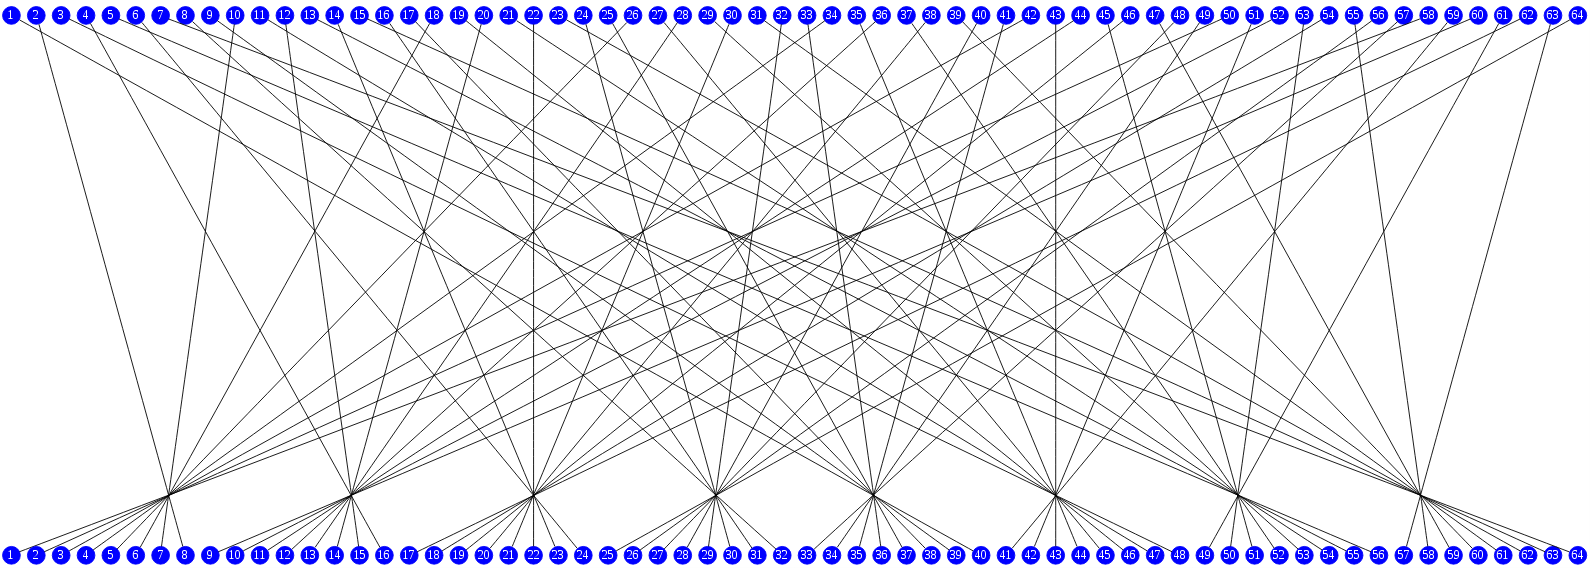
\includegraphics[width=16cm,height=7cm]{permutation}
\caption{A General Permutation}
\label{fig:permutation}
\end{figure}

\subsubsection{S-boxes}
An S-box is simply a look-up-table. In Serpent, the S-boxes are 4-bit permutations. The advantage of an S-box is that for a 1-bit change of an input value, the output is guaranteed to be altered by more than one bit (at least for the Serpent S-boxes). An exmaple S-box can be seen in Figure~\ref{fig:sbox}. Please note that this diagram does not represent the S-box for Serpent. The Serpent S-boxes can be seen in \cite{SERPENT}.

\begin{figure}[H]
\centering
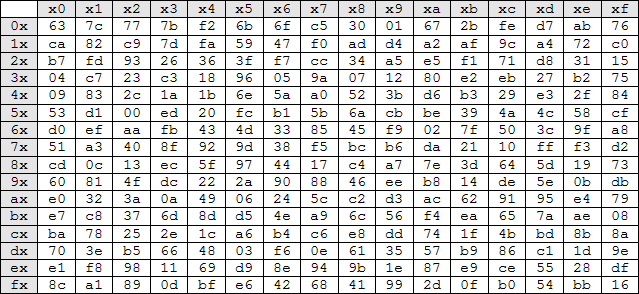
\includegraphics[width=16cm,height=7cm]{sbox}
\caption{A General S-box}
\label{fig:sbox}
\end{figure}

\subsubsection{Linear Transformation}
The linear transformation functions acts on the 128-bit block as four 32-bit words. Each word is linearly adjusted and combined with other words according to Figure~\ref{fig:linear}. In this figure, $<<<$ denotes a left rotation, and $<<$ denotes a left shift.

\begin{figure}[H]
\centering
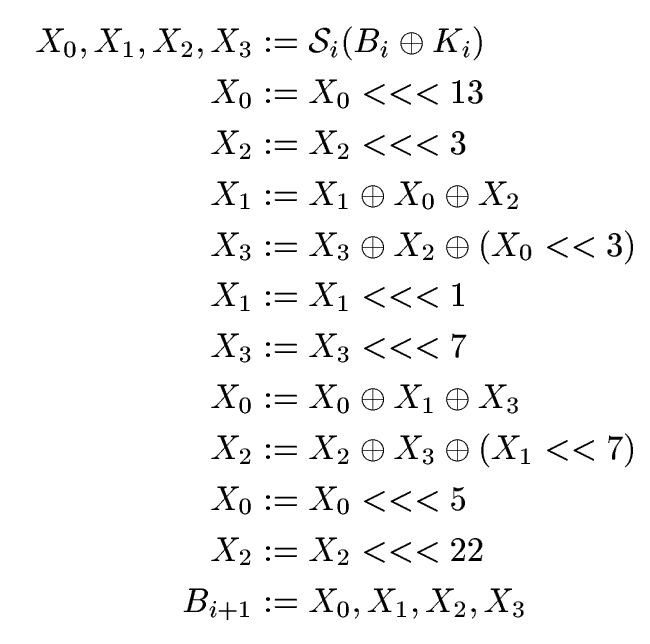
\includegraphics[width=7cm,height=7cm]{linear}
\caption{Linear Transformation}
\label{fig:linear}
\end{figure}

\begin{figure}[H]
\centering
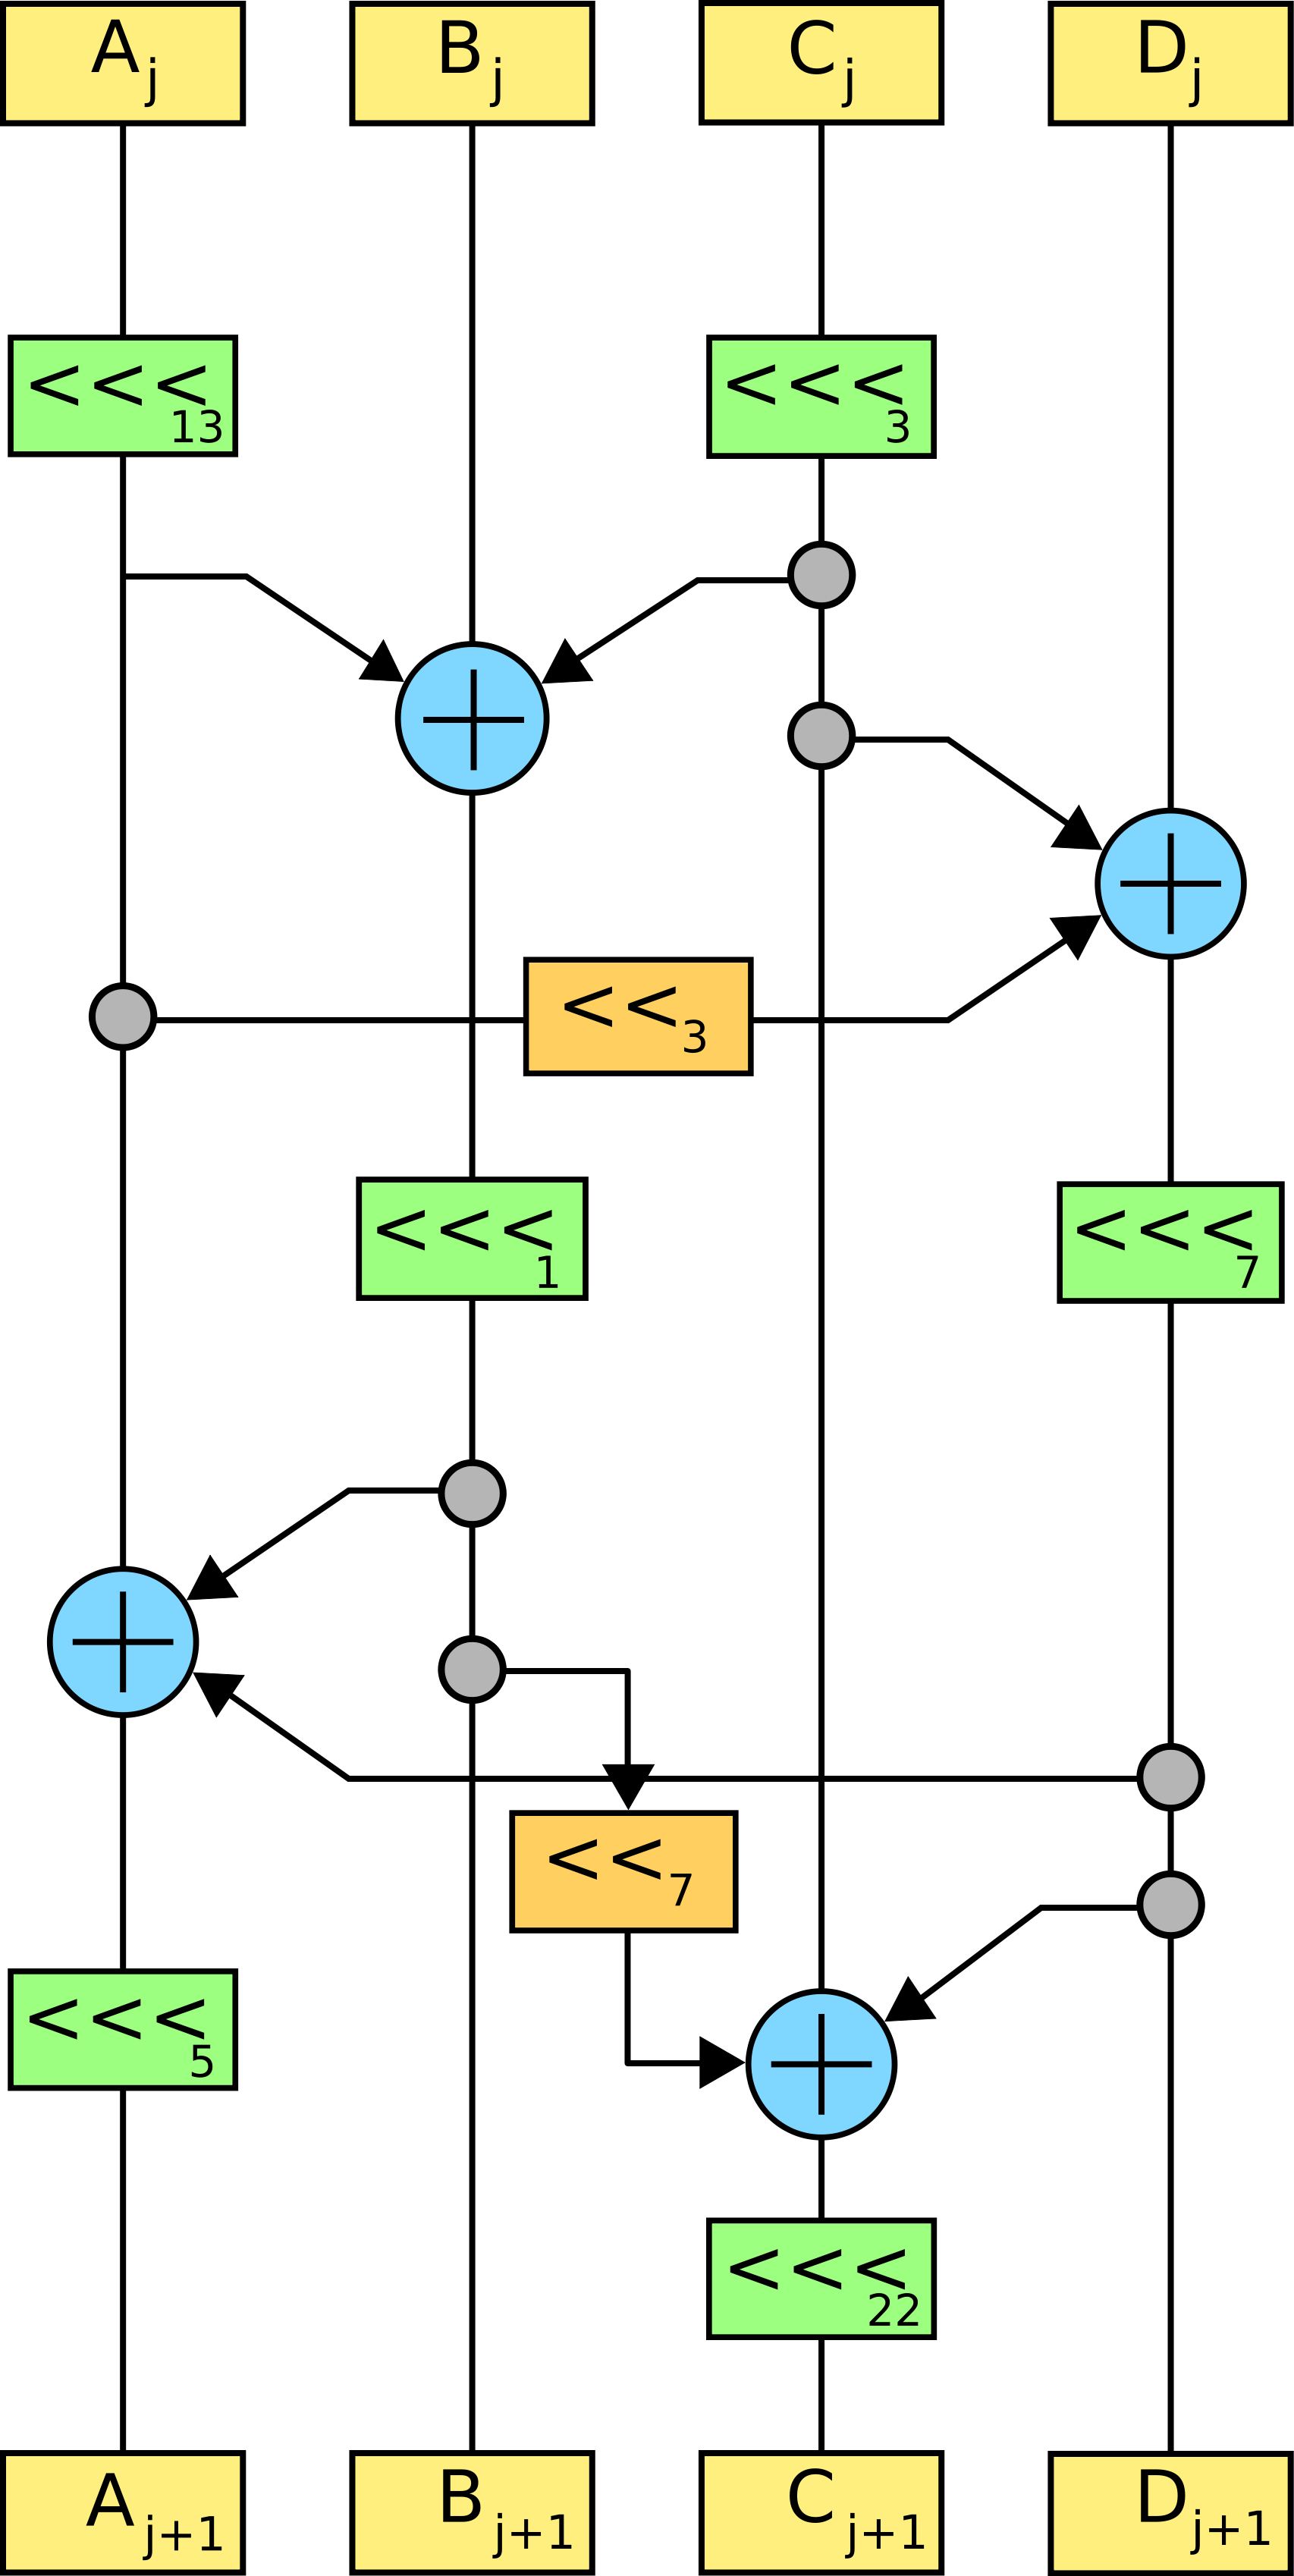
\includegraphics[width=7cm,height=11cm]{linear2}
\caption{Linear Transformation}
\label{fig:linear2}
\end{figure}


\subsubsection{Decryption}
Decrption is very similar to encryption. However, inverse S-boxes and linear transformations are used as well as a reverse order of subkeys. This is made most clear with the use of Figure~\ref{fig:decrypt}.

\begin{figure}[H]
\centering
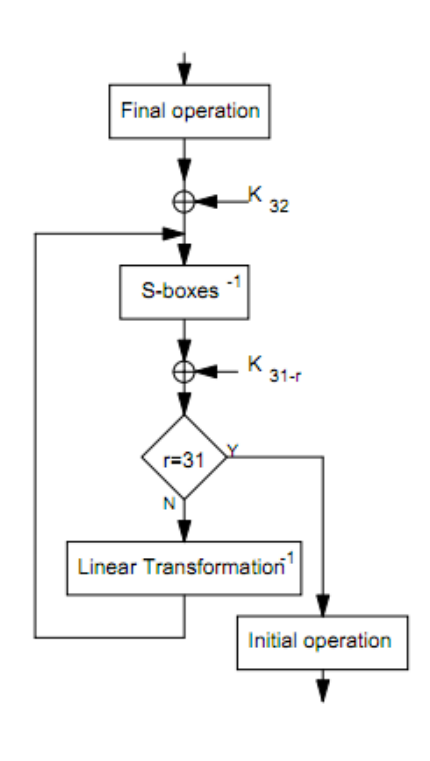
\includegraphics[width=7cm,height=11cm]{decrypt}
\caption{Block Diagram of the Decryption Process}
\label{fig:decrypt}
\end{figure}

%----------------------------------------------------------------------------------------
%	MAJOR SECTION 1
%----------------------------------------------------------------------------------------

\section{Original Implementation} % Major section
%------------------------------------------------
%------------------------------------------------
\subsection{Timing Results}
All timing results were measured on the CS machine, Joplin. Source-code level results were truncated as problem methods are easily identifiable within the first few lines.
\subsubsection{Total Running Time with no JIT compiler}
\$ time java -Xint Serpent 1     
\newline49672ba898d98df95019180445491089
\newline
real	0m0.135s
\newline
user	0m0.040s
\newline
sys	0m0.024s
\vfill
\subsubsection{Runtime Profiles of over 100 Seconds}

\$java -Xint -Xprof Serpent 100000
\newline d3f68d0623563be822d68dde8f4ad282
\newline Flat profile of 156.42 secs (15402 total ticks): main
\newline Interpreted \tab + \tab native \tab  Method                        
\newline  26.7\tab\%  4119\tab  +\tab     0\tab    Serpent.sBox
\newline  22.8\tab\%  3511\tab  +\tab     0\tab    Serpent.getRoundKey
\newline  21.4\tab\%  3290\tab  +\tab     0\tab    Serpent.initPermutation
\newline  21.3\tab\%  3274\tab  +\tab     0\tab    Serpent.linearTransform
\newline   3.5\tab\%   540\tab  +\tab     0\tab    Serpent.setKey
\newline   3.5\tab\%   537\tab  +\tab     0\tab    Serpent.finalPermutation
\newline   0.8\tab\%   128\tab  +\tab     0\tab    Serpent.encrypt
\newline   0.0\tab\%     0\tab  +\tab     2\tab    java.io.FileInputStream.readBytes
\newline   0.0\tab\%     0\tab  +\tab     1\tab    java.io.UnixFileSystem.getBooleanAttributes0
\newline 100.0\tab\% 15399\tab  +\tab     3\tab    Total interpreted
\newline\$time java -Xint -agentlib:hprof=cpu=samples,depth=10 Serpent 100000
\newline d3f68d0623563be822d68dde8f4ad282
\newline Dumping CPU usage by sampling running threads ... done.
\newline real	2m38.259s
\newline user	2m38.062s
\newline sys	0m0.488s
\newline rank\tab  self\tab\  accum\tab\    count\tab trace \tab method
\newline    1\tab  7.06\tab\%  7.06\tab\%    1092\tab 300041\tab Serpent.initPermutation
\newline    2\tab  6.91\tab\% 13.97\tab\%    1070\tab 300033\tab Serpent.linearTransform
\newline    3\tab  6.57\tab\% 20.54\tab\%    1016\tab 300042\tab Serpent.getRoundKey
\newline    4\tab  6.30\tab\% 26.84\tab\%     975\tab 300027\tab Serpent.sBox
\newline    5\tab  6.19\tab\% 33.03\tab\%     958\tab 300074\tab Serpent.initPermutation
\newline    6\tab  4.25\tab\% 37.27\tab\%     657\tab 300032\tab Serpent.sBox
\newline    7\tab  2.43\tab\% 39.70\tab\%     376\tab 300040\tab Serpent.initPermutation
\newline    8\tab  2.35\tab\% 42.05\tab\%     364\tab 300045\tab Serpent.initPermutation
\newline    9\tab  2.31\tab\% 44.36\tab\%     357\tab 300086\tab Serpent.finalPermutation
\newline   10\tab  2.29\tab\% 46.66\tab\%     355\tab 300034\tab Serpent.finalPermutation
\newline   11\tab  2.27\tab\% 48.93\tab\%     352\tab 300051\tab Serpent.initPermutation
%------------------------------------------------
\subsection{Analysis}
These timing results both show the major functions taking the majority of the CPU as expected. Namely, initPermutations. Logically, initial permutations should take very little time as it is only called once for each encryption. However, an implementation was made which uses the inital permutation of the linear transform of the final permutation (IP(LT(FP(x)))) as noted in \cite{SERPENT}.

\subsection{Example Runs}
\begin{lstlisting}
java Serpent 1
49672ba898d98df95019180445491089

java Serpent 100
5a445efd4923ebddea1d5be4511bd4d6

java Serpent 1000
d72ec2b7b93fbb567cefbab3fab43fb4

\end{lstlisting}
Each of these runs use a key of all ``0's" and a plaintext of all ``0's." Please note that these values match the values specified at: http://www.cs.technion.ac.il/~biham/Reports/Serpent/Serpent-256-128.verified.test-vectors
\section{Optimized Code}
The two most substantial optimizations made were to the functions initPermutation and finalPermutation. Both involved looping through every single bit in the data block, accessing values in lookup tables each time, and both functions are used many times, in the linearTransformation function as well as the getRoundKey function. The loops and lookup tables were eliminated from each function, assigning all the values directly instead, with one statement per byte in the block. This improved execution time by about 30\%. Other minor modifications were made across other functions to eliminate unnecessary looping or array creation.
\subsection{Timing Results}
\subsubsection{Total Running Time with no JIT compiler}
\subsubsection{Runtime Profiles of over 100 Seconds}
\subsection{Analysis}
\subsection{Example Runs}

\section{Division of Labor}
\begin{itemize}
 \item Nicholas Sereni
 \begin{itemize}
  \item{Linear Transform}
  \item{Final Report}
  \item{Runtime Results}
  \item{General Debugging}
 \end{itemize}
 \item{Dan Grau}
 \begin{itemize}
  \item{Initial and Final Permutations}
  \item{File Reading}
  \item{Optimizations}
  \item{General Debugging}
 \end{itemize}
 \item{Karl Berger}
 \begin{itemize}
  \item{Key Scheduler}
  \item{S-Boxes}
  \item{Decryption}
  \item{General Debugging}
 \end{itemize}
\end{itemize}

\section{Manuals}
\subsection{Developer's Guide}
  If the source code has been removed from the given archive, then all that is required is BlockCipher.java and Serpent.java (or SerpentOptimized.java to run the optimized code).  Execute the following command to compile the program:
  \begin{verbatim}
  	javac -classpath <path to Parallel Java library> BlockCipher.java Serpent.java
  \end{verbatim}
  
\subsection{User's Guide}
  Once the program has been compiled, there are two ways in which it can be run.  The first is to encrypt a block of 0s N number of times with a key of all 0s.
  \begin{verbatim}
  	java Serpent <N>
  \end{verbatim}
  The second way to run the program is the encrypt or decrypt a file.  There are 5 arguments to the program in this case and are as follows.
  \begin{verbatim}
  	java Serpent <input filename> <output filename> <key in hex> \
  	  <integer Nonce> <`e' to encrypt or `d' to decrypt>
  \end{verbatim}
  For example:
  \begin{verbatim}
  	java Serpent cat.jpg cat.encrypt 112233445566778899aabbccddeeff 12345 e
  \end{verbatim}

%------------------------------------------------
\section{Source Code}
\subsection{Original Code}
\begin{lstlisting}[language=Java, basicstyle=\small, breaklines=true]
import edu.rit.util.Hex;
import edu.rit.util.Packing;
import java.nio.ByteBuffer;
import java.nio.ByteOrder;
import java.util.Arrays;
import java.lang.Integer;
import java.io.*;

public class Serpent implements BlockCipher {

    private static final byte xFF = (byte)0xFF;
    private int keySize;
    private byte[] key;
    private int[] prekeys;

    public Serpent() {
        prekeys = new int[140];
    }

    /**
     * Returns this block cipher's block size in bytes.
     *
     * @return  Block size.
     */
    public int blockSize() {
        return 16;
    }

    /**
     * Returns this block cipher's key size in bytes.
     *
     * @return  Key size.
     */
    public int keySize() {
        return 32;
    }

    /**
     * Set the key for this block cipher. If <TT>key</TT> is an array of bytes
     * whose length is less than <TT>keySize()</TT>, it will be padded to 
     * <TT>keySize()</TT>
     *
     * @param  key  Key.
     */
    public void setKey(byte[] key) {
        if (key.length != keySize()) {
            this.key = new byte[keySize()];
            for( int i = 0; i < key.length; i++ ) {
                this.key[i] = key[i];
            }
			      //Pad key to 256-bit
            for( int i = key.length; i < keySize(); i++ ) {
                if( i == key.length ) {
                    //Start of padding!
                    this.key[i] = (byte)0x80;
                }else {
                    this.key[i] = (byte)0x00;
                }
            }
        }else {
            this.key = key;
        }

        //prekey initialization from K
        for(int i = 0; i < 8; i++) {
            prekeys[i] = Packing.packIntBigEndian(new byte[]{this.key[4*i],this.key[4*i+1],this.key[4*i+2],this.key[4*i+3]}, 0);
        }
        //Build out prekey array
		    //There's a shift of 8 positions here because I build the intermediate keys in the same
		    //array as the other prekeys.
        for( int i = 8; i < prekeys.length; i++ ) {
            byte[] prnt = new byte[4];
			      //Phi is the fractional part of the golden ratio
            int phi = 0x9e3779b9;
            int tmp;
            tmp = prekeys[i-8] ^ prekeys[i-5] ^ prekeys[i-3] ^ prekeys[i-1] ^ 
                i-8 ^ phi;
            prekeys[i] = (tmp << 11) | (tmp >>> (21));
            prnt = new byte[4];
            Packing.unpackIntBigEndian(prekeys[i], prnt, 0);
         }
    }


    
    /**
     * Encrypt the given plaintext. <TT>text</TT> must be an array of bytes
     * whose length is equal to <TT>blockSize()</TT>. On input, <TT>text</TT>
     * contains the plaintext block. The plaintext block is encrypted using the
     * key specified in the most recent call to <TT>setKey()</TT>. On output,
     * <TT>text</TT> contains the ciphertext block.
     *
     * @param  text  Plaintext (on input), ciphertext (on output).
     */
    public void encrypt(byte[] text) {
        byte[] data = initPermutation(text);
        byte[] temp = new byte[] {
                data[12], data[13], data[14], data[15],
                data[8], data[9], data[10], data[11],
                data[4], data[5], data[6], data[7],
                data[0], data[1], data[2], data[3],
                };
        data = temp;
        byte[] roundKey = new byte[16];
        //32 rounds
        for(int i = 0; i < 32; i++){
            roundKey = getRoundKey(i);
            for(int n = 0; n < 16; n++){
                data[n] = (byte) (data[n] ^ roundKey[n]);
            }
            data = sBox(data, i);
            
            if(i == 31){
				        //For round 32, instead of a linear transform
				        // we get the last produced round key and xor 
				        // it with the current state.
                roundKey = getRoundKey(32);
                for(int n = 0; n < 16; n++){
                    data[n] = (byte) (data[n] ^ roundKey[n]);
                } 
            }
            else{
                data = linearTransform(data);
            }
        }
        data = finalPermutation(data);   
        text[0] = data[3];
        text[1] = data[2];
        text[2] = data[1];
        text[3] = data[0];
        text[4] = data[7];
        text[5] = data[6];
        text[6] = data[5];
        text[7] = data[4];
        text[8] = data[11];
        text[9] = data[10];
        text[10] = data[9];
        text[11] = data[8];
        text[12] = data[15];
        text[13] = data[14];
        text[14] = data[13];
        text[15] = data[12];
    }

    /**
     * Decrypt the given ciphertext.  We decrypt by performing the inverse
	   * operations performed to encrypt in reverse order.
     *
     * @param  text  ciphertext (on input), original plaintext (on output).
     */
    public void decrypt(byte[] text) {
        byte[] temp = new byte[] {
                text[3], text[2], text[1], text[0],
                text[7], text[6], text[5], text[4],
                text[11], text[10], text[9], text[8],
                text[15], text[14], text[13], text[12],
            };
        byte[] data = initPermutation(temp);
        byte[] roundKey = getRoundKey(32);
        for(int n = 0; n < 16; n++){
            data[n] = (byte) (data[n] ^ roundKey[n]);
        }
        //32 rounds in reverse
        for(int i = 31; i >= 0; i--){
            if(i!=31){
                data = invLinearTransform(data);
            }
            data = sBoxInv(data, i);
            roundKey = getRoundKey(i);
            for(int n = 0; n < 16; n++){
                data[n] = (byte) (data[n] ^ roundKey[n]);
            }
        }
        data = finalPermutation(data);   
        text[0] = data[3];
        text[1] = data[2];
        text[2] = data[1];
        text[3] = data[0];
        text[4] = data[7];
        text[5] = data[6];
        text[6] = data[5];
        text[7] = data[4];
        text[8] = data[11];
        text[9] = data[10];
        text[10] = data[9];
        text[11] = data[8];
        text[12] = data[15];
        text[13] = data[14];
        text[14] = data[13];
        text[15] = data[12];
    }

    private byte[] initPermutation(byte[] data) {
        byte[] output = new byte[16];
        for (int i = 0;  i < 128; i++) {
			      //Bit permutation based on ip lookup table
            int bit = (data[(ipTable[i]) / 8] >>> ((ipTable[i]) % 8)) & 0x01;
            if ((bit & 0x01) == 1)
                output[15- (i/8)] |= 1 << (i % 8);
            else
                output[15 - (i/8)] &= ~(1 << (i % 8));
        }
        return output; 
    }

    private byte[] finalPermutation(byte[] data) {
        byte[] output = new byte[16];
        for (int i = 0;  i < 128; i++) {
			      //Bit permutation based on fp lookup table
            int bit = (data[15-fpTable[i] / 8] >>> (fpTable[i] % 8)) & 0x01;
            if ((bit & 0x01) == 1)
                output[(i/8)] |= 1 << (i % 8);
            else
                output[(i/8)] &= ~(1 << (i % 8));
        }
        return output; 
    }

    private static byte[] s0 = new byte[]
        {3,8,15,1,10,6,5,11,14,13,4,2,7,0,9,12};
    private static byte[] s1 = new byte[]
        {15,12,2,7,9,0,5,10,1,11,14,8,6,13,3,4};
    private static byte[] s2 = new byte[]
        {8,6,7,9,3,12,10,15,13,1,14,4,0,11,5,2};
    private static byte[] s3 = new byte[]
        {0,15,11,8,12,9,6,3,13,1,2,4,10,7,5,14};
    private static byte[] s4 = new byte[]
        {1,15,8,3,12,0,11,6,2,5,4,10,9,14,7,13};
    private static byte[] s5 = new byte[]
        {15,5,2,11,4,10,9,12,0,3,14,8,13,6,7,1};
    private static byte[] s6 = new byte[]
        {7,2,12,5,8,4,6,11,14,9,1,15,13,3,10,0};
    private static byte[] s7 = new byte[]
        {1,13,15,0,14,8,2,11,7,4,12,10,9,3,5,6};
    private static byte[][] sBoxes = new byte[][]
        {s0,s1,s2,s3,s4,s5,s6,s7};

    /**
     * Perform S-Box manipulation to the given byte array of <TT>blocksize()</TT> length.
     *
     * @param data Input bit sequence
     * @param round Number of the current round, used to determine which S-Box to use.
     */
    private byte[] sBox(byte[] data, int round) {
        byte[] toUse = sBoxes[round%8];
        byte[] output = new byte[blockSize()];
        for( int i = 0; i < blockSize(); i++ ) {
            //Break signed-ness
            int curr = data[i]&0xFF;
            byte low4 = (byte)(curr>>>4);
            byte high4 = (byte)(curr&0x0F);
            output[i] = (byte) ((toUse[low4]<<4) ^ (toUse[high4]));
        }
        return output;
    }

    private static byte[] is0 = new byte[]
        {13,3,11,0,10,6,5,12,1,14,4,7,15,9,8,2};
    private static byte[] is1 = new byte[]
        {5,8,2,14,15,6,12,3,11,4,7,9,1,13,10,0};
    private static byte[] is2 = new byte[]
        {12,9,15,4,11,14,1,2,0,3,6,13,5,8,10,7};
    private static byte[] is3 = new byte[]
        {0,9,10,7,11,14,6,13,3,5,12,2,4,8,15,1};
    private static byte[] is4 = new byte[]
        {5,0,8,3,10,9,7,14,2,12,11,6,4,15,13,1};
    private static byte[] is5 = new byte[]
        {8,15,2,9,4,1,13,14,11,6,5,3,7,12,10,0};
    private static byte[] is6 = new byte[]
        {15,10,1,13,5,3,6,0,4,9,14,7,2,12,8,11};
    private static byte[] is7 = new byte[]
        {3,0,6,13,9,14,15,8,5,12,11,7,10,1,4,2};
    private static byte[][] isBoxes = new byte[][]
        {is0,is1,is2,is3,is4,is5,is6,is7};    

    /**
     * Perform inverse S-Box manipulation to the given byte array of <TT>blocksize()</TT> length.
     *
     * @param data Input bit sequence
     * @param round Number of the current round, used to determine which inverted S-Box to use.
     */
    private byte[] sBoxInv(byte[] data, int round) {
        byte[] toUse = isBoxes[round%8];
        byte[] output = new byte[blockSize()];
        for( int i = 0; i < blockSize(); i++ ) {
            //Break signed-ness
            int curr = data[i]&0xFF;
            byte low4 = (byte)(curr>>>4);
            byte high4 = (byte)(curr&0x0F);
            output[i] = (byte) ((toUse[low4]<<4) ^ (toUse[high4]));
        }
        return output;
    }

    private static byte[] ipTable = new byte[] {
         0, 32, 64,  96,  1, 33, 65,  97,  2, 34, 66,  98,  3, 35, 67,  99,
         4, 36, 68, 100,  5, 37, 69, 101,  6, 38, 70, 102,  7, 39, 71, 103,
         8, 40, 72, 104,  9, 41, 73, 105, 10, 42, 74, 106, 11, 43, 75, 107,
        12, 44, 76, 108, 13, 45, 77, 109, 14, 46, 78, 110, 15, 47, 79, 111,
        16, 48, 80, 112, 17, 49, 81, 113, 18, 50, 82, 114, 19, 51, 83, 115,
        20, 52, 84, 116, 21, 53, 85, 117, 22, 54, 86, 118, 23, 55, 87, 119,
        24, 56, 88, 120, 25, 57, 89, 121, 26, 58, 90, 122, 27, 59, 91, 123,
        28, 60, 92, 124, 29, 61, 93, 125, 30, 62, 94, 126, 31, 63, 95, 127
    };

    private static byte[] fpTable = new byte[] {
         0,  4,  8, 12, 16, 20, 24, 28, 32,  36,  40,  44,  48,  52,  56,  60,
        64, 68, 72, 76, 80, 84, 88, 92, 96, 100, 104, 108, 112, 116, 120, 124,
         1,  5,  9, 13, 17, 21, 25, 29, 33,  37,  41,  45,  49,  53,  57,  61,
        65, 69, 73, 77, 81, 85, 89, 93, 97, 101, 105, 109, 113, 117, 121, 125,
         2,  6, 10, 14, 18, 22, 26, 30, 34,  38,  42,  46,  50,  54,  58,  62,
        66, 70, 74, 78, 82, 86, 90, 94, 98, 102, 106, 110, 114, 118, 122, 126,
         3,  7, 11, 15, 19, 23, 27, 31, 35,  39,  43,  47,  51,  55,  59,  63,
        67, 71, 75, 79, 83, 87, 91, 95, 99, 103, 107, 111, 115, 119, 123, 127
    };
    
    /**
     * Performs linear transformation on the input bit sequence
     * 
     * @param data Input bit sequence
     * @return output bit sequence
     */
    private byte[] linearTransform(byte[] data){
        data = finalPermutation(data);
        byte[] output = new byte[blockSize()];
        ByteBuffer buffer = ByteBuffer.wrap(data);
        int x0 =  buffer.getInt();
        int x1 =  buffer.getInt();
        int x2 =  buffer.getInt();
        int x3 =  buffer.getInt();
        x0 = ((x0 << 13) | (x0 >>> (32 - 13))); 
        x2 = ((x2 << 3) | (x2 >>> (32 - 3)));
        x1 = x1 ^ x0 ^ x2;
        x3 = x3 ^ x2 ^ (x0 << 3);
        x1 = (x1 << 1) | (x1 >>> (32 - 1));
        x3 = (x3 << 7) | (x3 >>> (32 - 7));
        x0 = x0 ^ x1 ^ x3;
        x2 = x2 ^ x3 ^ (x1 << 7);
        x0 = (x0 << 5) | (x0 >>> (32-5));
        x2 = (x2 << 22) | (x2 >>> (32-22));
        buffer.clear();
        buffer.putInt(x0);
        buffer.putInt(x1);
        buffer.putInt(x2);
        buffer.putInt(x3);
        
        output = buffer.array();
        output = initPermutation(output);
        
        return output;
    }

    /**
     * Performs inverse linear transformation on the input bit sequence.
	   * This is the linear transform in reverse with inverted operations.
     * 
     * @param data Input bit sequence
     * @return output bit sequence
     */
    private byte[] invLinearTransform(byte[] data){
        data = finalPermutation(data);
        byte[] output = new byte[blockSize()];
        ByteBuffer buffer = ByteBuffer.wrap(data);
        int x0 =  buffer.getInt();
        int x1 =  buffer.getInt();
        int x2 =  buffer.getInt();
        int x3 =  buffer.getInt();

        x2 = (x2 >>> 22) | (x2 << (32-22));
        x0 = (x0 >>> 5) | (x0 << (32-5));
        x2 = x2 ^ x3 ^ (x1 << 7);
        x0 = x0 ^ x1 ^ x3;
        x3 = (x3 >>> 7) | (x3 << (32-7));
        x1 = (x1 >>> 1) | (x1 << (32-1));
        x3 = x3 ^ x2 ^ (x0 << 3);
        x1 = x1 ^ x0 ^ x2;
        x2 = (x2 >>> 3) | (x2 << (32-3));
        x0 = (x0 >>> 13) | (x0 << (32-13));
        
        buffer.clear();
        buffer.putInt(x0);
        buffer.putInt(x1);
        buffer.putInt(x2);
        buffer.putInt(x3);

        output = buffer.array();
        output = initPermutation(output);

        return output;
    }

	/**
	 * Fetches round key.  Round keys are built on request from the
	 * prekeys that were created when the key was set.
	 *
	 * @param round Number of the round for which a key is needed.
	 * @return byte[] The round key for the requested round.
	 */
    private byte[] getRoundKey(int round) {
        int k0 = prekeys[4*round+8];
        int k1 = prekeys[4*round+9];
        int k2 = prekeys[4*round+10];
        int k3 = prekeys[4*round+11];
        int box = (((3-round)%8)+8)%8;
        byte[] in = new byte[16];
        for (int j = 0; j < 32; j+=2) {
            in[j/2] = (byte) (((k0 >>> j) & 0x01)     |
            ((k1 >>> j) & 0x01) << 1 |
            ((k2 >>> j) & 0x01) << 2 |
            ((k3 >>> j) & 0x01) << 3 |
            ((k0 >>> j+1) & 0x01) << 4 |
            ((k1 >>> j+1) & 0x01) << 5 |
            ((k2 >>> j+1) & 0x01) << 6 |
            ((k3 >>> j+1) & 0x01) << 7 );
        }
        byte[] out = sBox(in, box);
        byte[] key = new byte[16];
        for (int i = 3; i >= 0; i--) {
            for(int j = 0; j < 4; j++) {
                key[3-i] |= (out[i*4+j] & 0x01) << (j*2) | ((out[i*4+j] >>> 4) & 0x01) << (j*2+1) ;
                key[7-i] |= ((out[i*4+j] >>> 1) & 0x01) << (j*2) | ((out[i*4+j] >>> 5) & 0x01) << (j*2+1) ;
                key[11-i] |= ((out[i*4+j] >>> 2) & 0x01) << (j*2) | ((out[i*4+j] >>> 6) & 0x01) << (j*2+1) ;
                key[15-i] |= ((out[i*4+j] >>> 3) & 0x01) << (j*2) | ((out[i*4+j] >>> 7) & 0x01) << (j*2+1) ;
            }
        }
        return initPermutation(key);
    }
}
\end{lstlisting}
\subsection{Optimized Code}
\begin{lstlisting}[language=Java, basicstyle=\small, breaklines=true]
import edu.rit.util.Hex;
import edu.rit.util.Packing;
import java.nio.ByteBuffer;
import java.nio.ByteOrder;
import java.util.Arrays;
import java.lang.Integer;
import java.io.*;

public class SerpentOptimized implements BlockCipher {

    private static final byte xFF = (byte)0xFF;
	private int keySize;
    private byte[] key;
    private int[] prekeys;

    public SerpentOptimized() {
        prekeys = new int[140];
    }

    /**
     * Returns this block cipher's block size in bytes.
     *
     * @return  Block size.
     */
    public int blockSize() {
        return 16;
    }

    /**
     * Returns this block cipher's key size in bytes.
     *
     * @return  Key size.
     */
    public int keySize() {
        return 32;
    }

    /**
     * Set the key for this block cipher. If <TT>key</TT> is an array of bytes
     * whose length is less than <TT>keySize()</TT>, it will be padded to 
     * <TT>keySize()</TT>
     *
     * @param  key  Key.
     */
    public void setKey(byte[] key) {
        if (key.length != keySize()) {
            this.key = new byte[keySize()];
            for( int i = 0; i < key.length; i++ ) {
                this.key[i] = key[i];
            }
            for( int i = key.length; i < keySize(); i++ ) {
                if( i == key.length ) {
                    //Start of padding!
                    this.key[i] = (byte)0x80;
                }else {
                    this.key[i] = (byte)0x00;
                }
            }
        }else {
            this.key = key;
        }

        //prekey initialization from K
        for(int i = 0; i < 8; i++) {
            prekeys[i] = Packing.packIntBigEndian(new byte[]{this.key[4*i],this.key[4*i+1],this.key[4*i+2],this.key[4*i+3]}, 0);
        }
        //Build out prekey array
        for( int i = 8; i < prekeys.length; i++ ) {
            byte[] prnt = new byte[4];
            int phi = 0x9e3779b9;
            //(x << n) | (x >>> (32 - n)) Rotate
            int tmp;
            tmp = prekeys[i-8] ^ prekeys[i-5] ^ prekeys[i-3] ^ prekeys[i-1] ^ 
                i-8 ^ phi;
            prekeys[i] = (tmp << 11) | (tmp >>> (21));
            prnt = new byte[4];
            Packing.unpackIntBigEndian(prekeys[i], prnt, 0);
         }
    }


    
    /**
     * Encrypt the given plaintext. <TT>text</TT> must be an array of bytes
     * whose length is equal to <TT>blockSize()</TT>. On input, <TT>text</TT>
     * contains the plaintext block. The plaintext block is encrypted using the
     * key specified in the most recent call to <TT>setKey()</TT>. On output,
     * <TT>text</TT> contains the ciphertext block.
     *
     * @param  text  Plaintext (on input), ciphertext (on output).
     */
    public void encrypt(byte[] text) {
		byte[] data = initPermutation(text);
		//System.out.println(Hex.toString(data));
		byte[] temp = new byte[] {
				data[12], data[13], data[14], data[15],
				data[8], data[9], data[10], data[11],
				data[4], data[5], data[6], data[7],
				data[0], data[1], data[2], data[3],
				};
		data = temp;
        byte[] roundKey = new byte[16];
        //32 rounds
        for(int i = 0; i < 32; i++){
            roundKey = getRoundKey(i);
           // System.out.println("key:"+Hex.toString(roundKey));
            for(int n = 0; n < 16; n++){
                data[n] = (byte) (data[n] ^ roundKey[n]);
            }
          //  System.out.println(Hex.toString(data));
            data = sBox(data, i);
          //  System.out.println(Hex.toString(data));
            
            if(i == 31){
            	roundKey = getRoundKey(32);
                for(int n = 0; n < 16; n++){
                    data[n] = (byte) (data[n] ^ roundKey[n]);
                } 
            }
            else{
            	data = linearTransform(data);
          //  	System.out.println(Hex.toString(data));
            }
        }
        data = finalPermutation(data);   
        text[0] = data[3];
        text[1] = data[2];
        text[2] = data[1];
        text[3] = data[0];
        text[4] = data[7];
        text[5] = data[6];
        text[6] = data[5];
        text[7] = data[4];
        text[8] = data[11];
        text[9] = data[10];
        text[10] = data[9];
        text[11] = data[8];
        text[12] = data[15];
        text[13] = data[14];
        text[14] = data[13];
        text[15] = data[12];
    }

    /**
     * Decrypt the given ciphertext.  We decrypt by performing the inverse
     * operations performed to encrypt in reverse order.
     *
     * @param  text  ciphertext (on input), original plaintext (on output).
     */
    public void decrypt(byte[] text) {
        byte[] temp = new byte[] {
                text[3], text[2], text[1], text[0],
                text[7], text[6], text[5], text[4],
                text[11], text[10], text[9], text[8],
                text[15], text[14], text[13], text[12],
            };
        byte[] data = initPermutation(temp);
        byte[] roundKey = getRoundKey(32);
        for(int n = 0; n < 16; n++){
            data[n] = (byte) (data[n] ^ roundKey[n]);
        }
        //32 rounds in reverse
        for(int i = 31; i >= 0; i--){
            if(i!=31){
                data = invLinearTransform(data);
            }
            data = sBoxInv(data, i);
            roundKey = getRoundKey(i);
            for(int n = 0; n < 16; n++){
                data[n] = (byte) (data[n] ^ roundKey[n]);
            }
        }
        data = finalPermutation(data);   
        text[0] = data[3];
        text[1] = data[2];
        text[2] = data[1];
        text[3] = data[0];
        text[4] = data[7];
        text[5] = data[6];
        text[6] = data[5];
        text[7] = data[4];
        text[8] = data[11];
        text[9] = data[10];
        text[10] = data[9];
        text[11] = data[8];
        text[12] = data[15];
        text[13] = data[14];
        text[14] = data[13];
        text[15] = data[12];
    }

    /**
     * Perform initial permutation on the input
     *
     * @param data Input bit sequence
     */
    private byte[] initPermutation(byte[] input) {
        byte[] output = new byte[16];
        output[15] = (byte) ((((input[0] & 0x01))) | (((input[4])& 0x01) << 1) | (((input[8])& 0x01) << 2) | (((input[12])& 0x01) << 3) | 
                     (((input[0]>>>1)& 0x01) << 4) | (((input[4]>>>1)& 0x01) << 5) | (((input[8]>>>1)& 0x01) << 6) | (((input[12]>>>1)& 0x01) << 7));
        output[14] = (byte) ((((input[0]>>>2 & 0x01))) | (((input[4]>>>2)& 0x01) << 1) | (((input[8]>>>2)& 0x01) << 2) | (((input[12]>>>2)& 0x01) << 3) | 
                     (((input[0]>>>3)& 0x01) << 4) | (((input[4]>>>3)& 0x01) << 5) | (((input[8]>>>3)& 0x01) << 6) | (((input[12]>>>3)& 0x01) << 7));
        output[13] = (byte) ((((input[0]>>>4 & 0x01))) | (((input[4]>>>4)& 0x01) << 1) | (((input[8]>>>4)& 0x01) << 2) | (((input[12]>>>4)& 0x01) << 3) | 
                     (((input[0]>>>5)& 0x01) << 4) | (((input[4]>>>5)& 0x01) << 5) | (((input[8]>>>5)& 0x01) << 6) | (((input[12]>>>5)& 0x01) << 7));
        output[12] = (byte) ((((input[0]>>>6 & 0x01))) | (((input[4]>>>6)& 0x01) << 1) | (((input[8]>>>6)& 0x01) << 2) | (((input[12]>>>6)& 0x01) << 3) | 
                    (((input[0]>>>7)& 0x01) << 4) | (((input[4]>>>7)& 0x01) << 5) | (((input[8]>>>7)& 0x01) << 6) | (((input[12]>>>7)& 0x01) << 7));
        
        output[11] = (byte) ((((input[1] & 0x01))) | (((input[5])& 0x01) << 1) | (((input[9])& 0x01) << 2) | (((input[13])& 0x01) << 3) | 
                    (((input[1]>>>1)& 0x01) << 4) | (((input[5]>>>1)& 0x01) << 5) | (((input[9]>>>1)& 0x01) << 6) | (((input[13]>>>1)& 0x01) << 7));
        output[10] = (byte) ((((input[1]>>>2 & 0x01))) | (((input[5]>>>2)& 0x01) << 1) | (((input[9]>>>2)& 0x01) << 2) | (((input[13]>>>2)& 0x01) << 3) | 
                    (((input[1]>>>3)& 0x01) << 4) | (((input[5]>>>3)& 0x01) << 5) | (((input[9]>>>3)& 0x01) << 6) | (((input[13]>>>3)& 0x01) << 7));
        output[9] = (byte) ((((input[1]>>>4 & 0x01))) | (((input[5]>>>4)& 0x01) << 1) | (((input[9]>>>4)& 0x01) << 2) | (((input[13]>>>4)& 0x01) << 3) | 
                    (((input[1]>>>5)& 0x01) << 4) | (((input[5]>>>5)& 0x01) << 5) | (((input[9]>>>5)& 0x01) << 6) | (((input[13]>>>5)& 0x01) << 7));
        output[8] = (byte) ((((input[1]>>>6 & 0x01))) | (((input[5]>>>6)& 0x01) << 1) | (((input[9]>>>6)& 0x01) << 2) | (((input[13]>>>6)& 0x01) << 3) | 
                    (((input[1]>>>7)& 0x01) << 4) | (((input[5]>>>7)& 0x01) << 5) | (((input[9]>>>7)& 0x01) << 6) | (((input[13]>>>7)& 0x01) << 7));
        
        output[7] = (byte) ((((input[2] & 0x01))) | (((input[6])& 0x01) << 1) | (((input[10])& 0x01) << 2) | (((input[14])& 0x01) << 3) | 
                    (((input[2]>>>1)& 0x01) << 4) | (((input[6]>>>1)& 0x01) << 5) | (((input[10]>>>1)& 0x01) << 6) | (((input[14]>>>1)& 0x01) << 7));
        output[6] = (byte) ((((input[2]>>>2 & 0x01))) | (((input[6]>>>2)& 0x01) << 1) | (((input[10]>>>2)& 0x01) << 2) | (((input[14]>>>2)& 0x01) << 3) | 
                    (((input[2]>>>3)& 0x01) << 4) | (((input[6]>>>3)& 0x01) << 5) | (((input[10]>>>3)& 0x01) << 6) | (((input[14]>>>3)& 0x01) << 7));
        output[5] = (byte) ((((input[2]>>>4 & 0x01))) | (((input[6]>>>4)& 0x01) << 1) | (((input[10]>>>4)& 0x01) << 2) | (((input[14]>>>4)& 0x01) << 3) | 
                    (((input[2]>>>5)& 0x01) << 4) | (((input[6]>>>5)& 0x01) << 5) | (((input[10]>>>5)& 0x01) << 6) | (((input[14]>>>5)& 0x01) << 7));
        output[4] = (byte) ((((input[2]>>>6 & 0x01))) | (((input[6]>>>6)& 0x01) << 1) | (((input[10]>>>6)& 0x01) << 2) | (((input[14]>>>6)& 0x01) << 3) | 
                    (((input[2]>>>7)& 0x01) << 4) | (((input[6]>>>7)& 0x01) << 5) | (((input[10]>>>7)& 0x01) << 6) | (((input[14]>>>7)& 0x01) << 7));

        output[3] = (byte) ((((input[3] & 0x01))) | (((input[7])& 0x01) << 1) | (((input[11])& 0x01) << 2) | (((input[15])& 0x01) << 3) | 
                    (((input[3]>>>1)& 0x01) << 4) | (((input[7]>>>1)& 0x01) << 5) | (((input[11]>>>1)& 0x01) << 6) | (((input[15]>>>1)& 0x01) << 7));
        output[2] = (byte) ((((input[3]>>>2 & 0x01))) | (((input[7]>>>2)& 0x01) << 1) | (((input[11]>>>2)& 0x01) << 2) | (((input[15]>>>2)& 0x01) << 3) | 
                    (((input[3]>>>3)& 0x01) << 4) | (((input[7]>>>3)& 0x01) << 5) | (((input[11]>>>3)& 0x01) << 6) | (((input[15]>>>3)& 0x01) << 7));
        output[1] = (byte) ((((input[3]>>>4 & 0x01))) | (((input[7]>>>4)& 0x01) << 1) | (((input[11]>>>4)& 0x01) << 2) | (((input[15]>>>4)& 0x01) << 3) | 
                    (((input[3]>>>5)& 0x01) << 4) | (((input[7]>>>5)& 0x01) << 5) | (((input[11]>>>5)& 0x01) << 6) | (((input[15]>>>5)& 0x01) << 7));
        output[0] = (byte) ((((input[3]>>>6 & 0x01))) | (((input[7]>>>6)& 0x01) << 1) | (((input[11]>>>6)& 0x01) << 2) | (((input[15]>>>6)& 0x01) << 3) | 
                    (((input[3]>>>7)& 0x01) << 4) | (((input[7]>>>7)& 0x01) << 5) | (((input[11]>>>7)& 0x01) << 6) | (((input[15]>>>7)& 0x01) << 7));
                    
        return output; 
    }

    /**
     * Perform finalls
      permutation on the input
     *
     * @param data Input bit sequence
     */
    private byte[] finalPermutation(byte[] input) {
        byte[] output = new byte[16];
        output[0] = (byte) ((((input[15]>>>0) & 0x01)) | (((input[15]>>>4)& 0x01) << 1) | (((input[14]>>>0)& 0x01) << 2) | (((input[14]>>>4)& 0x01) << 3) | 
                     (((input[13]>>>0)& 0x01) << 4) | (((input[13]>>>4)& 0x01) << 5) | (((input[12]>>>0)& 0x01) << 6) | (((input[12]>>>4)& 0x01) << 7));
        output[1] = (byte) ((((input[11]>>>0) & 0x01)) | (((input[11]>>>4)& 0x01) << 1) | (((input[10]>>>0)& 0x01) << 2) | (((input[10]>>>4)& 0x01) << 3) | 
                     (((input[9]>>>0)& 0x01) << 4) | (((input[9]>>>4)& 0x01) << 5) | (((input[8]>>>0)& 0x01) << 6) | (((input[8]>>>4)& 0x01) << 7));
        output[2] = (byte) ((((input[7]>>>0) & 0x01)) | (((input[7]>>>4)& 0x01) << 1) | (((input[6]>>>0)& 0x01) << 2) | (((input[6]>>>4)& 0x01) << 3) | 
                     (((input[5]>>>0)& 0x01) << 4) | (((input[5]>>>4)& 0x01) << 5) | (((input[4]>>>0)& 0x01) << 6) | (((input[4]>>>4)& 0x01) << 7));
        output[3] = (byte) ((((input[3]>>>0) & 0x01)) | (((input[3]>>>4)& 0x01) << 1) | (((input[2]>>>0)& 0x01) << 2) | (((input[2]>>>4)& 0x01) << 3) | 
                    (((input[1]>>>0)& 0x01) << 4) | (((input[1]>>>4)& 0x01) << 5) | (((input[0]>>>0)& 0x01) << 6) | (((input[0]>>>4)& 0x01) << 7));
        
        output[4] = (byte) ((((input[15]>>>1) & 0x01)) | (((input[15]>>>5)& 0x01) << 1) | (((input[14]>>>1)& 0x01) << 2) | (((input[14]>>>5)& 0x01) << 3) | 
                     (((input[13]>>>1)& 0x01) << 4) | (((input[13]>>>5)& 0x01) << 5) | (((input[12]>>>1)& 0x01) << 6) | (((input[12]>>>5)& 0x01) << 7));
        output[5] = (byte) ((((input[11]>>>1) & 0x01)) | (((input[11]>>>5)& 0x01) << 1) | (((input[10]>>>1)& 0x01) << 2) | (((input[10]>>>5)& 0x01) << 3) | 
                     (((input[9]>>>1)& 0x01) << 4) | (((input[9]>>>5)& 0x01) << 5) | (((input[8]>>>1)& 0x01) << 6) | (((input[8]>>>5)& 0x01) << 7));
        output[6] = (byte) ((((input[7]>>>1) & 0x01)) | (((input[7]>>>5)& 0x01) << 1) | (((input[6]>>>1)& 0x01) << 2) | (((input[6]>>>5)& 0x01) << 3) | 
                     (((input[5]>>>1)& 0x01) << 4) | (((input[5]>>>5)& 0x01) << 5) | (((input[4]>>>1)& 0x01) << 6) | (((input[4]>>>5)& 0x01) << 7));
        output[7] = (byte) ((((input[3]>>>1) & 0x01)) | (((input[3]>>>5)& 0x01) << 1) | (((input[2]>>>1)& 0x01) << 2) | (((input[2]>>>5)& 0x01) << 3) | 
                    (((input[1]>>>1)& 0x01) << 4) | (((input[1]>>>5)& 0x01) << 5) | (((input[0]>>>1)& 0x01) << 6) | (((input[0]>>>5)& 0x01) << 7));

        output[8] = (byte) ((((input[15]>>>2) & 0x01)) | (((input[15]>>>6)& 0x01) << 1) | (((input[14]>>>2)& 0x01) << 2) | (((input[14]>>>6)& 0x01) << 3) | 
                     (((input[13]>>>2)& 0x01) << 4) | (((input[13]>>>6)& 0x01) << 5) | (((input[12]>>>2)& 0x01) << 6) | (((input[12]>>>6)& 0x01) << 7));
        output[9] = (byte) ((((input[11]>>>2) & 0x01)) | (((input[11]>>>6)& 0x01) << 1) | (((input[10]>>>2)& 0x01) << 2) | (((input[10]>>>6)& 0x01) << 3) | 
                     (((input[9]>>>2)& 0x01) << 4) | (((input[9]>>>6)& 0x01) << 5) | (((input[8]>>>2)& 0x01) << 6) | (((input[8]>>>6)& 0x01) << 7));
        output[10] = (byte) ((((input[7]>>>2) & 0x01)) | (((input[7]>>>6)& 0x01) << 1) | (((input[6]>>>2)& 0x01) << 2) | (((input[6]>>>6)& 0x01) << 3) | 
                     (((input[5]>>>2)& 0x01) << 4) | (((input[5]>>>6)& 0x01) << 5) | (((input[4]>>>2)& 0x01) << 6) | (((input[4]>>>6)& 0x01) << 7));
        output[11] = (byte) ((((input[3]>>>2) & 0x01)) | (((input[3]>>>6)& 0x01) << 1) | (((input[2]>>>2)& 0x01) << 2) | (((input[2]>>>6)& 0x01) << 3) | 
                    (((input[1]>>>2)& 0x01) << 4) | (((input[1]>>>6)& 0x01) << 5) | (((input[0]>>>2)& 0x01) << 6) | (((input[0]>>>6)& 0x01) << 7));

        output[12] = (byte) ((((input[15]>>>3) & 0x01)) | (((input[15]>>>7)& 0x01) << 1) | (((input[14]>>>3)& 0x01) << 2) | (((input[14]>>>7)& 0x01) << 3) | 
                     (((input[13]>>>3)& 0x01) << 4) | (((input[13]>>>7)& 0x01) << 5) | (((input[12]>>>3)& 0x01) << 6) | (((input[12]>>>7)& 0x01) << 7));
        output[13] = (byte) ((((input[11]>>>3) & 0x01)) | (((input[11]>>>7)& 0x01) << 1) | (((input[10]>>>3)& 0x01) << 2) | (((input[10]>>>7)& 0x01) << 3) | 
                     (((input[9]>>>3)& 0x01) << 4) | (((input[9]>>>7)& 0x01) << 5) | (((input[8]>>>3)& 0x01) << 6) | (((input[8]>>>7)& 0x01) << 7));
        output[14] = (byte) ((((input[7]>>>3) & 0x01)) | (((input[7]>>>7)& 0x01) << 1) | (((input[6]>>>3)& 0x01) << 2) | (((input[6]>>>7)& 0x01) << 3) | 
                     (((input[5]>>>3)& 0x01) << 4) | (((input[5]>>>7)& 0x01) << 5) | (((input[4]>>>3)& 0x01) << 6) | (((input[4]>>>7)& 0x01) << 7));
        output[15] = (byte) ((((input[3]>>>3) & 0x01)) | (((input[3]>>>7)& 0x01) << 1) | (((input[2]>>>3)& 0x01) << 2) | (((input[2]>>>7)& 0x01) << 3) | 
                    (((input[1]>>>3)& 0x01) << 4) | (((input[1]>>>7)& 0x01) << 5) | (((input[0]>>>3)& 0x01) << 6) | (((input[0]>>>7)& 0x01) << 7));

    	return output; 
    }

    private static byte[] s0 = new byte[]
        {3,8,15,1,10,6,5,11,14,13,4,2,7,0,9,12};
    private static byte[] s1 = new byte[]
        {15,12,2,7,9,0,5,10,1,11,14,8,6,13,3,4};
    private static byte[] s2 = new byte[]
        {8,6,7,9,3,12,10,15,13,1,14,4,0,11,5,2};
    private static byte[] s3 = new byte[]
        {0,15,11,8,12,9,6,3,13,1,2,4,10,7,5,14};
    private static byte[] s4 = new byte[]
        {1,15,8,3,12,0,11,6,2,5,4,10,9,14,7,13};
    private static byte[] s5 = new byte[]
        {15,5,2,11,4,10,9,12,0,3,14,8,13,6,7,1};
    private static byte[] s6 = new byte[]
        {7,2,12,5,8,4,6,11,14,9,1,15,13,3,10,0};
    private static byte[] s7 = new byte[]
        {1,13,15,0,14,8,2,11,7,4,12,10,9,3,5,6};
    private static byte[][] sBoxes = new byte[][]
        {s0,s1,s2,s3,s4,s5,s6,s7};

    /**
     * Perform S-Box manipulation to the given byte array of <TT>blocksize()</TT> length.
     *
     * @param data Input bit sequence
     * @param round Number of the current round, used to determine which S-Box to use.
     */
    private byte[] sBox(byte[] data, int round) {
        byte[] toUse = sBoxes[round%8];
        byte[] output = new byte[blockSize()];
        for( int i = 0; i < blockSize(); i++ ) {
            //Break signed-ness
            int curr = data[i]&0xFF;
            byte low4 = (byte)(curr>>>4);
            byte high4 = (byte)(curr&0x0F);
            output[i] = (byte) ((toUse[low4]<<4) ^ (toUse[high4]));
        }
        return output;
    }

    private static byte[] is0 = new byte[]
        {13,3,11,0,10,6,5,12,1,14,4,7,15,9,8,2};
    private static byte[] is1 = new byte[]
        {5,8,2,14,15,6,12,3,11,4,7,9,1,13,10,0};
    private static byte[] is2 = new byte[]
        {12,9,15,4,11,14,1,2,0,3,6,13,5,8,10,7};
    private static byte[] is3 = new byte[]
        {0,9,10,7,11,14,6,13,3,5,12,2,4,8,15,1};
    private static byte[] is4 = new byte[]
        {5,0,8,3,10,9,7,14,2,12,11,6,4,15,13,1};
    private static byte[] is5 = new byte[]
        {8,15,2,9,4,1,13,14,11,6,5,3,7,12,10,0};
    private static byte[] is6 = new byte[]
        {15,10,1,13,5,3,6,0,4,9,14,7,2,12,8,11};
    private static byte[] is7 = new byte[]
        {3,0,6,13,9,14,15,8,5,12,11,7,10,1,4,2};
    private static byte[][] isBoxes = new byte[][]
        {is0,is1,is2,is3,is4,is5,is6,is7};    

    /**
     * Perform inverse S-Box manipulation to the given byte array of <TT>blocksize()</TT> length.
     *
     * @param data Input bit sequence
     * @param round Number of the current round, used to determine which inverted S-Box to use.
     */
    private byte[] sBoxInv(byte[] data, int round) {
        byte[] toUse = isBoxes[round%8];
        byte[] output = new byte[blockSize()];
        for( int i = 0; i < blockSize(); i++ ) {
            //Break signed-ness
            int curr = data[i]&0xFF;
            byte low4 = (byte)(curr>>>4);
            byte high4 = (byte)(curr&0x0F);
            output[i] = (byte) ((toUse[low4]<<4) ^ (toUse[high4]));
        }
        return output;
    }
    
    /**
     * Performs linear transformation on the input bit sequence
     * 
     * @param data Input bit sequence
     * @return output bit sequence
     */
    private byte[] linearTransform(byte[] data){
    	data = finalPermutation(data);
    	//byte[] output = new byte[blockSize()];
    	ByteBuffer buffer = ByteBuffer.wrap(data);
    	//buffer.order(ByteOrder.LITTLE_ENDIAN);
    	int x0 =  buffer.getInt();
    	int x1 =  buffer.getInt();
    	int x2 =  buffer.getInt();
    	int x3 =  buffer.getInt();
    	x0 = ((x0 << 13) | (x0 >>> (32 - 13)));	
    	x2 = ((x2 << 3) | (x2 >>> (32 - 3)));
    	x1 = x1 ^ x0 ^ x2;
    	x3 = x3 ^ x2 ^ (x0 << 3);
    	x1 = (x1 << 1) | (x1 >>> (32 - 1));
    	x3 = (x3 << 7) | (x3 >>> (32 - 7));
    	x0 = x0 ^ x1 ^ x3;
    	x2 = x2 ^ x3 ^ (x1 << 7);
    	x0 = (x0 << 5) | (x0 >>> (32-5));
    	x2 = (x2 << 22) | (x2 >>> (32-22));
    	buffer.clear();
    	buffer.putInt(x0);
    	buffer.putInt(x1);
    	buffer.putInt(x2);
    	buffer.putInt(x3);
    	
    	data = buffer.array();
    	data = initPermutation(data);
    	
    	return data;
    }

    /**
     * Performs inverse linear transformation on the input bit sequence.
     * This is the linear transform in reverse with inverted operations.
     * 
     * @param data Input bit sequence
     * @return output bit sequence
     */
    private byte[] invLinearTransform(byte[] data){
        data = finalPermutation(data);
        ByteBuffer buffer = ByteBuffer.wrap(data);
        int x0 =  buffer.getInt();
        int x1 =  buffer.getInt();
        int x2 =  buffer.getInt();
        int x3 =  buffer.getInt();

        x2 = (x2 >>> 22) | (x2 << (32-22));
        x0 = (x0 >>> 5) | (x0 << (32-5));
        x2 = x2 ^ x3 ^ (x1 << 7);
        x0 = x0 ^ x1 ^ x3;
        x3 = (x3 >>> 7) | (x3 << (32-7));
        x1 = (x1 >>> 1) | (x1 << (32-1));
        x3 = x3 ^ x2 ^ (x0 << 3);
        x1 = x1 ^ x0 ^ x2;
        x2 = (x2 >>> 3) | (x2 << (32-3));
        x0 = (x0 >>> 13) | (x0 << (32-13));
        
        buffer.clear();
        buffer.putInt(x0);
        buffer.putInt(x1);
        buffer.putInt(x2);
        buffer.putInt(x3);

        data = buffer.array();
        data = initPermutation(data);

        return data;
    }

    /**
     * Fetches round key.  Round keys are built on request from the
     * prekeys that were created when the key was set.
     *
     * @param round Number of the round for which a key is needed.
     * @return byte[] The round key for the requested round.
     */
    private byte[] getRoundKey(int round) {
        int k0 = prekeys[4*round+8];
        int k1 = prekeys[4*round+9];
        int k2 = prekeys[4*round+10];
        int k3 = prekeys[4*round+11];
        int box = (((3-round)%8)+8)%8;
        byte[] in = new byte[16];
        for (int j = 0; j < 32; j+=2) {
            in[j/2] = (byte) (((k0 >>> j) & 0x01)     |
            ((k1 >>> j) & 0x01) << 1 |
            ((k2 >>> j) & 0x01) << 2 |
            ((k3 >>> j) & 0x01) << 3 |
            ((k0 >>> j+1) & 0x01) << 4 |
            ((k1 >>> j+1) & 0x01) << 5 |
            ((k2 >>> j+1) & 0x01) << 6 |
            ((k3 >>> j+1) & 0x01) << 7 );
        }
        byte[] out = sBox(in, box);
        byte[] key = new byte[16];
        for (int i = 3; i >= 0; i--) {
            for(int j = 0; j < 4; j++) {
                key[3-i] |= (out[i*4+j] & 0x01) << (j*2) | ((out[i*4+j] >>> 4) & 0x01) << (j*2+1) ;
                key[7-i] |= ((out[i*4+j] >>> 1) & 0x01) << (j*2) | ((out[i*4+j] >>> 5) & 0x01) << (j*2+1) ;
                key[11-i] |= ((out[i*4+j] >>> 2) & 0x01) << (j*2) | ((out[i*4+j] >>> 6) & 0x01) << (j*2+1) ;
                key[15-i] |= ((out[i*4+j] >>> 3) & 0x01) << (j*2) | ((out[i*4+j] >>> 7) & 0x01) << (j*2+1) ;
            }
        }
        return initPermutation(key);
    }

    /**
     * Main function, does one of two things:
     * sets an all-zero-byte key, performs N encryptions of an all-zero-byte plaintext block
     * or 
     * encrypts the contents of the input file, storing the result in an output file
     * args either specifies N or 
     * input filename, output filename, key (up to 32 bytes in hex), nonce (integer), and [e]ncrypt or [d]ecrypt
     */
    public static void main( String[] args ) {
        Serpent serpent = new Serpent();
        if(args.length == 1)
        {
            byte[] test_in = new byte[] {
                0x00,0x00,0x00,0x00,0x00,0x00,0x00,0x00,
                0x00,0x00,0x00,0x00,0x00,0x00,0x00,0x00,
            };
            byte[] test_key = new byte[] {
                0x00,0x00,0x00,0x00,0x00,0x00,0x00,0x00,
                0x00,0x00,0x00,0x00,0x00,0x00,0x00,0x00,
                0x00,0x00,0x00,0x00,0x00,0x00,0x00,0x00,
                0x00,0x00,0x00,0x00,0x00,0x00,0x00,0x00
            };
            int iters = Integer.parseInt(args[0]);
            for(int n = 0; n < iters; n++){
                serpent.setKey(test_key);
                serpent.encrypt(test_in);
            }
            System.out.println(Hex.toString(test_in));
            
        }
        else if (args.length == 5) {
            //read file
            try{
            File file_in = new File(args[0]);
            byte [] fileData = new byte[(int)file_in.length()];
            DataInputStream in_stream = new DataInputStream((new FileInputStream(file_in)));
            in_stream.readFully(fileData);
            in_stream.close();
            byte[] key = Hex.toByteArray(args[2]);
            //set key
            serpent.setKey(key);
            //setup file writing
            File file_out = new File(args[1]);
            DataOutputStream out_stream = new DataOutputStream((new FileOutputStream(file_out)));
            byte[] iv = new byte[16];
            //Create Nonce from 4th argument.
            Packing.unpackIntLittleEndian(Integer.parseInt(args[3]),iv,0);
            serpent.encrypt(iv);
            //File encryption in CBC mode
            if(args[4].equals("e")) {
                for(int i = 0; i < fileData.length; i+=16){
                    byte[] block = new byte[] {
                        0x00,0x00,0x00,0x00,0x00,0x00,0x00,0x00,
                        0x00,0x00,0x00,0x00,0x00,0x00,0x00,0x00
                    };
                    for(int n = 0; n < 16 && i+n < fileData.length; n++){
                        block[n] = (byte) (fileData[i+n] ^ iv[n]);
                    }
                    serpent.encrypt(block);
                    iv = block;
                    out_stream.write(block, 0, block.length);
                }
            }
            //File decryption in CBC mode
            else if(args[4].equals("d")) {
                for(int i = 0; i < fileData.length; i+=16){
                    byte[] block = new byte[] {
                        0x00,0x00,0x00,0x00,0x00,0x00,0x00,0x00,
                        0x00,0x00,0x00,0x00,0x00,0x00,0x00,0x00
                    };
                    for(int n = 0; n < 16 && n < fileData.length; n++){
                        block[n] = (byte) (fileData[i+n]);
                    }
                    byte[] savedForIV = Arrays.copyOf(block,16);
                    serpent.decrypt(block);
                    for(int n = 0; n < 16; n++){
                        block[n] = (byte) (block[n] ^ iv[n]);
                    }
                    iv = savedForIV;
                    out_stream.write(block, 0, block.length);
                }
            }
            else {
                System.out.println("Encrypt/Decrypt option invalid, input e or d as 5th argument.");
            }
            out_stream.close();
            }
            catch(IOException e){
              System.err.println(e.getMessage());
            }
        }
    }
}//Serpent.java
\end{lstlisting}
%----------------------------------------------------------------------------------------
%	BIBLIOGRAPHY
%----------------------------------------------------------------------------------------

\begin{thebibliography}{99} % Bibliography - this is intentionally simple in this template

\bibitem[Anderson, R., Biham, E., \& Knudsen, L. 1998]{SERPENT}
Anderson, R., Biham, E., \& Knudsen, L. (1998).
\newblock Serpent: A proposal for the advanced encryption standard.
\newblock {\em NIST AES Proposal}, 1–23. Retrieved from ftp://ftp-prod-srv04.it.su.se/pub/security/docs/crypt/Ross\_Anderson/serpent.pdf

\end{thebibliography}

%----------------------------------------------------------------------------------------

\end{document}
